\section{Bilag}
\newgeometry{top=2cm, right=2cm, bottom=2cm, left=2cm}
\begin{figure}
    \caption{Vores projekt backlog dokument}
    \makebox[\textwidth]{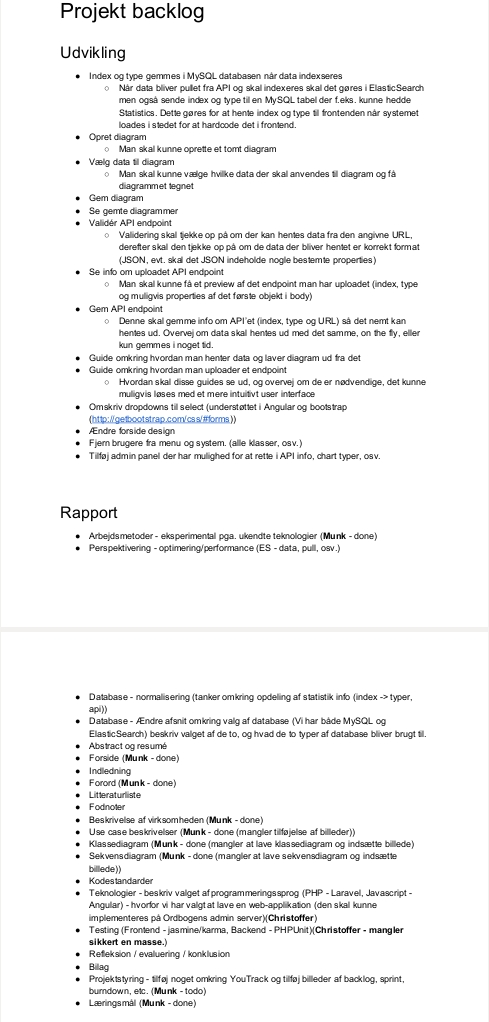
\includegraphics[scale=0.7]{Projekt_backlog}}
    \label{fig:projekt-backlog}
\end{figure}
\begin{landscape}
    \begin{figure}[H]
        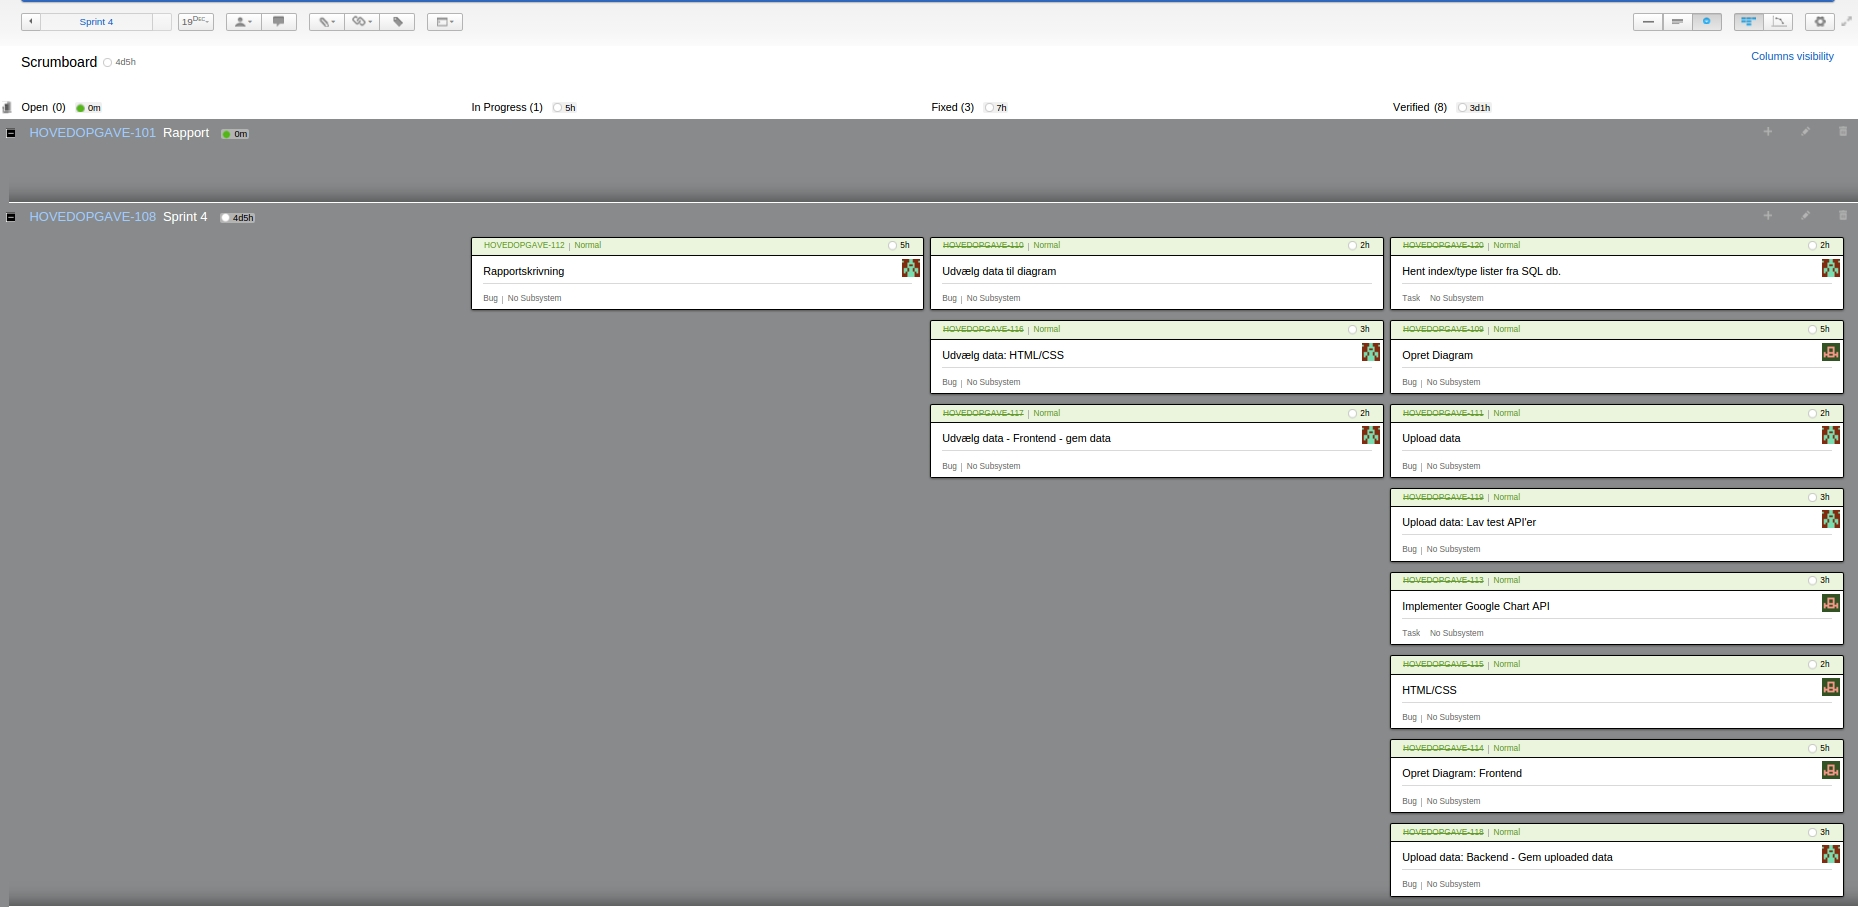
\includegraphics[scale=0.42]{Swim_lane}
        \caption{Swim lane fra sprint 4}
        \label{fig:swim-lane}
    \end{figure}
    \begin{figure}[H]
        \makebox{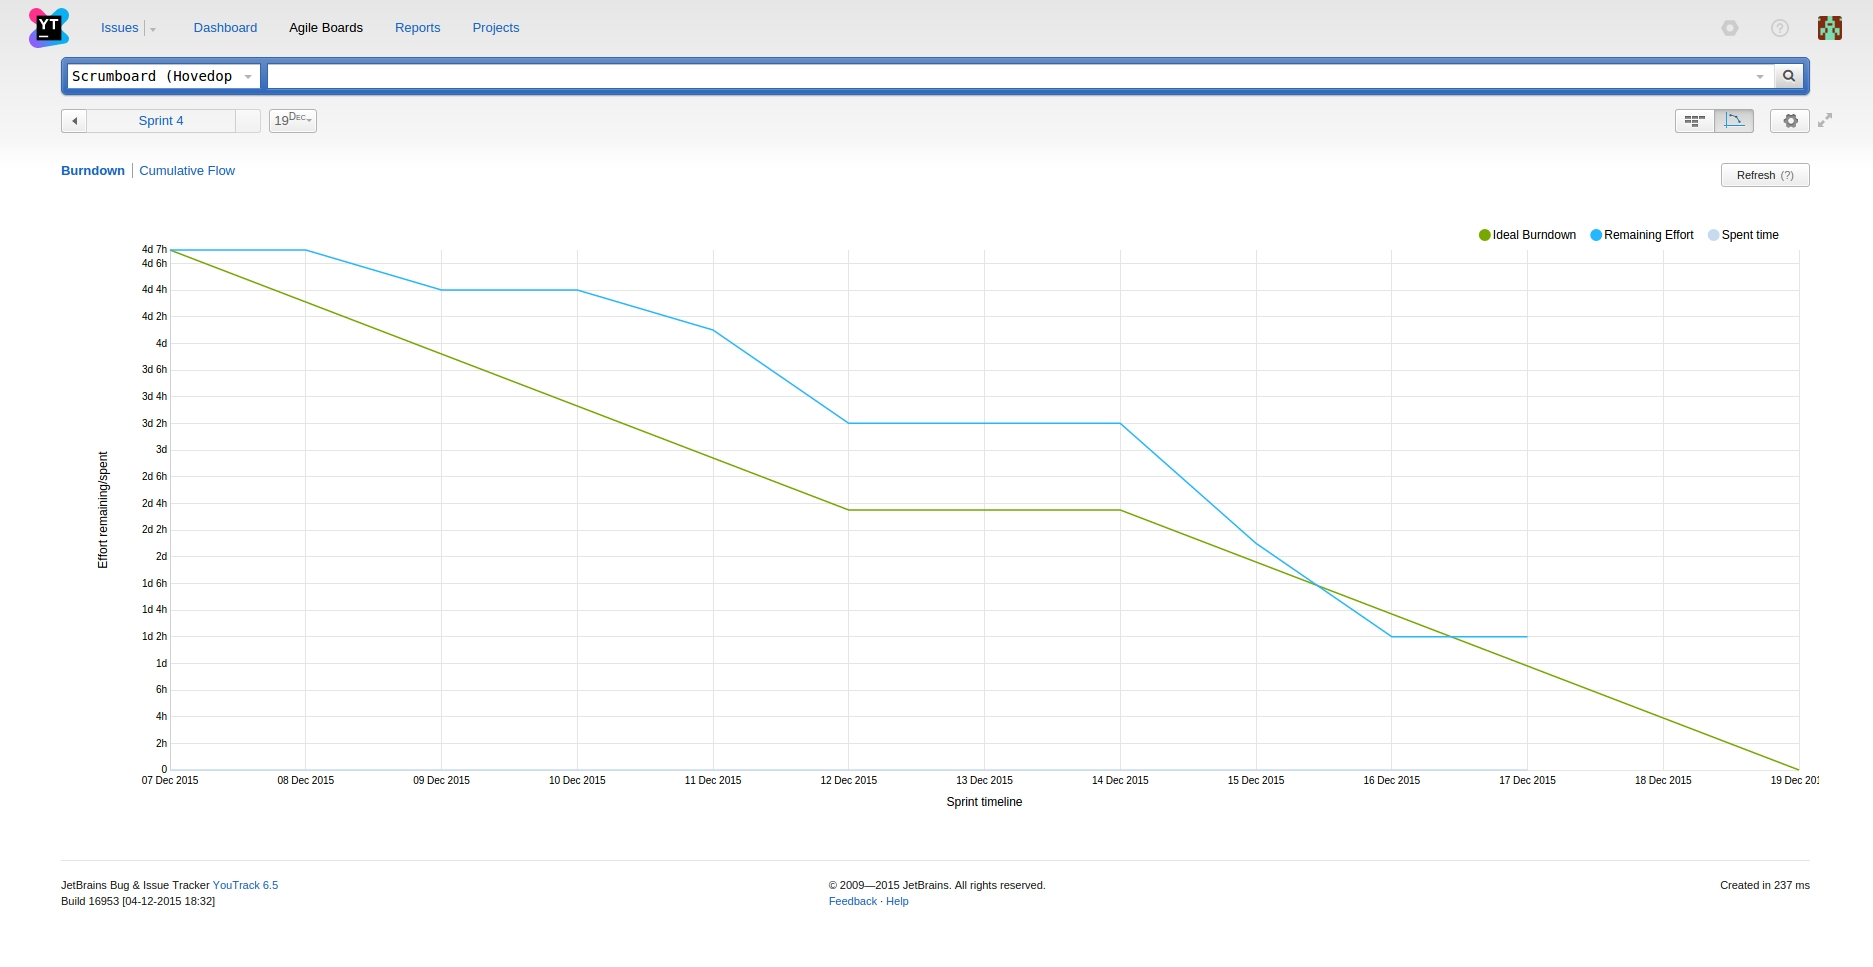
\includegraphics[scale=0.41]{Burndown_chart}}
        \caption{Burndown chart fra sprint 4}
        \label{fig:burndown-chart}
    \end{figure}
\end{landscape}
